\documentclass[11pt]{article}

\usepackage[T1]{fontenc}
\usepackage{mathtools,amsthm,amssymb}
\usepackage{lmodern}
\usepackage{microtype}
\usepackage[margin=1.05in]{geometry}
\usepackage{enumitem}
\usepackage{needspace}
\usepackage{xcolor}
\usepackage{tikz}
\usetikzlibrary{arrows.meta}
\pdftrailerid{}
\pdfsuppressptexinfo=15
\usepackage{hyperref}
\hypersetup{colorlinks=true,linkcolor=black,citecolor=black,
  urlcolor=blue!45!black,pdftitle={The second Kahn--Kalai conjecture}}

\newtheorem{theorem}{Theorem}[section]
\newtheorem{lemma}[theorem]{Lemma}
\numberwithin{equation}{section}
\theoremstyle{remark}
\newtheorem*{remark}{Remark}

\newcommand{\PP}{\mathbb P}
\newcommand{\EE}{\mathbb E}
\newcommand{\pc}{p_{\mathrm c}}
\newcommand{\pE}{p_{\mathrm E}}
\newcommand{\ind}{\mathbf 1}
\newcommand{\TT}{\mathcal T}
\newcommand{\UU}{\mathcal U}
\newcommand{\ch}{\operatorname{Ch}}
\newcommand{\ee}{\mathrm e}
\newcommand{\unverified}[1]{\par\smallskip\noindent\fbox{\parbox{0.95\linewidth}{\textbf{Unverified step.} #1}}\par\smallskip}
\newcommand{\step}[1]{\par\medskip\noindent\textbf{#1}\ }

\title{The second Kahn--Kalai conjecture}
\author{Rewritten for readability from the OpenAI manuscript of the same title}
\date{September 24, 2026}

\begin{document}
\maketitle
\begin{abstract}
For every finite simple graph $H$ with $h\ge1$ edges and at most $n$
vertices, the threshold for $G(n,p)$ to contain a copy of $H$ is at most
$C\,p_{\mathrm E}(n,H)(1+\log_2 h)$ with $C=2048\ee^{50}$, where
$p_{\mathrm E}(n,H)$ is the least density at which every subgraph of $H$
has expected copy count at least one half. This is the second
Kahn--Kalai conjecture. The present text is a step-by-step rewrite of
the source manuscript. One statement of the source, the
change-of-measure bound \eqref{eq:distortion} in Lemma~\ref{lem:local},
is claimed in greater generality than its proof supports; it is flagged
where it occurs. The restricted form that the proof does give is the
only form used later.
\end{abstract}

\section{The result}\label{sec:introduction}

\subsection{Setting and statement}

All graphs are finite and simple. For graphs $G$ and $F$, write $N(G,F)$
for the number of subgraphs of $G$ isomorphic to $F$. These are ordinary
copies: extra edges of $G$ between the chosen vertices are allowed. Let
$G(n,p)$ be the random graph on $[n]=\{1,\ldots,n\}$ in which each of
the $\binom n2$ possible edges is present independently with probability
$p$. A fixed copy of $F$ in the complete graph $K_n$ is present in
$G(n,p)$ with probability $p^{e(F)}$, so
\begin{equation}\label{eq:first-moment}
 \EE N(G(n,p),F)=N(K_n,F)\,p^{e(F)} .
\end{equation}
For a graph $H$ with at least one edge and at most $n$ vertices, define
\begin{align*}
 \pc(n,H)
 &=\inf\{p\in[0,1]:\PP(N(G(n,p),H)>0)\ge\tfrac12\},\\
 \pE(n,H)
 &=\inf\{p\in[0,1]:\EE N(G(n,p),F)\ge\tfrac12
                 \text{ for every subgraph }F\subseteq H\}.
\end{align*}
The first is the \emph{containment threshold}, the second the
\emph{graph expectation threshold}. Three elementary facts are used
later.
\begin{enumerate}[label=(\alph*),leftmargin=2em,itemsep=2pt]
 \item \emph{Both infima are attained.} The probability
 $\PP(N(G(n,p),H)>0)$ and each expectation \eqref{eq:first-moment} are
 polynomials in $p$, hence continuous. There are finitely many
 constraints, so each set is closed. Each set contains $p=1$, because
 $K_n$ contains $H$ and therefore every $F\subseteq H$.
 \item $\pE(n,H)>0$: for the single-edge subgraph the constraint reads
 $\binom n2p\ge\frac12$, which fails at $p=0$.
 \item $\pE(n,H)\le\pc(n,H)$: at $p=\pc(n,H)$ and for every
 $F\subseteq H$,
 $\EE N(G(n,p),F)\ge\PP(N(G(n,p),F)>0)\ge\PP(N(G(n,p),H)>0)\ge\frac12$.
\end{enumerate}

\begin{theorem}\label{thm:main}
For every $n\ge2$ and every finite simple graph $H$ with $h=e(H)\ge1$
edges and at most $n$ vertices,
\begin{equation}\label{eq:stronger}
 \pc(n,H)\le
 \min\{1,\;2048\ee^{50}\pE(n,H)(1+\log_2 h)\}.
\end{equation}
In particular,
\[
 \pc(n,H)\le6144\ee^{50}\pE(n,H)\log_2 n.
\]
\end{theorem}

Here $\ee$ is the base of the natural logarithm. The constants are
explicit and universal, and $H$ may vary with $n$.

\begin{remark}[Normalization]
Kahn and Kalai use expected count one rather than one half. By
\eqref{eq:first-moment}, the expected count of a subgraph with $x\ge1$
edges is proportional to $p^x$, so replacing $\frac12$ by $1$ changes
its constraint by the factor $2^{1/x}\le2$. The graph expectation
threshold therefore changes by a factor between one and two, and the
conjecture is the same.
\end{remark}

\begin{remark}[Why a logarithm is needed]
Let $H$ be a perfect matching on an even number $n$ of vertices. Then
$\pE(n,H)=\Theta(1/n)$, whereas
$\pc(n,H)=\Theta(\log n/n)$~\cite{ER66,KK07}: the larger scale is needed
to eliminate isolated vertices of the host. Hamilton cycles exhibit the
same logarithmic gap~\cite{KK07}.
\end{remark}

\subsection{Proof at a glance}\label{sec:glance}

Put $X=\binom{[n]}2$. The edge set of $G(n,p)$ is a random subset
$W\subseteq X$ with law $\mu_p$, meaning that each element is included
independently with probability $p$. A random set $A\subseteq X$ is
\emph{$a$-spread} if $\PP(J\subseteq A)\le a^{|J|}$ for every nonempty
$J\subseteq X$.

\paragraph{Key idea.}
Build $H$ in stages $\varnothing=H_0\subset H_1\subset\cdots\subset H_k=H$,
and record \emph{all} ways of extending a copy of $H_{i-1}$ in $K_n$ to
a copy of $H_i$ in a rooted tree. The arc labels are the added edge
sets. A single random set $W$ is then used to shrink the labels at every
node of the tree at once. Reusing $W$ across levels is legitimate
because the labels along one root-to-leaf path are pairwise disjoint.

\paragraph{Steps.}
\begin{enumerate}[label=\arabic*.,leftmargin=2em,itemsep=3pt]
 \item \emph{Lemma~\ref{lem:local} (local resampling), one family.}
 Given an $a$-spread family of sets of size at most $m$ and
 $W\sim\mu_\rho$ with $\rho=\ee^{50}a$, a randomized rule selects a
 member $A_b$ (the ``target'') such that $|A_b\setminus W|\le m/2$
 except with probability $\ee^{-9m}$. A second estimate
 \eqref{eq:distortion} says that selecting $b$ distorts the law of
 functions of $W$ outside $A_b$ by a factor at most $\ee^{11m}$.
 \item \emph{Lemma~\ref{lem:reduction} (reduction), the whole tree.}
 Apply Step~1 at every node with the same $W$. With probability at
 least $\frac34$ one obtains a subtree whose labels are the old labels
 minus $W$, with all capacities halved and spread parameters multiplied
 by at most $(1-\ee^{-m_j})^{-1}$. The proof uses both parts of
 Lemma~\ref{lem:local} and the disjointness of labels along paths.
 \item \emph{Theorem~\ref{thm:tree} (tree covering).} Iterate Step~2.
 After $\lfloor\log_2\ell_k\rfloor+1$ successes every label is empty, so
 the union of the sets $W$ used contains all labels of one path of the
 original tree. This costs density
 $16\ee^{50}\sigma(1+\log_2\ell_k)$.
 \item \emph{Lemma~\ref{lem:hierarchy} (graph hierarchy).} From $H$,
 construct such a tree with spread $\sigma=128\,\pE(n,H)$ and largest
 label size $\ell_k\le e(H)$. The definition of $\pE$ enters only here.
 \item \emph{Theorem~\ref{thm:main}} is Theorem~\ref{thm:tree} applied
 to the tree of Lemma~\ref{lem:hierarchy}.
\end{enumerate}

\begin{center}
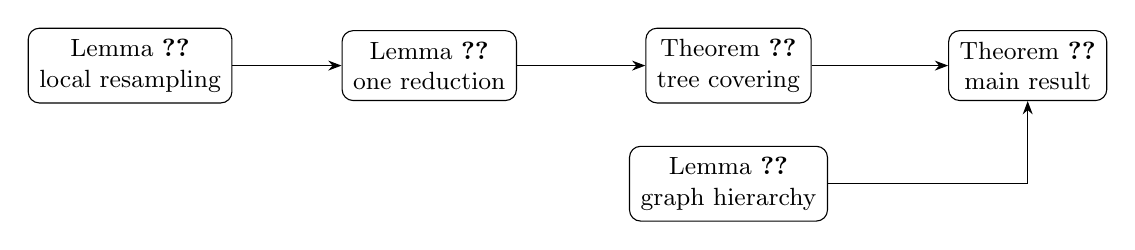
\begin{tikzpicture}[>=Stealth,
  box/.style={draw,rounded corners,inner sep=4pt,font=\small,align=center}]
\node[box] (L21) at (0,0) {Lemma~\ref{lem:local}\\local resampling};
\node[box] (L32) at (3.8,0) {Lemma~\ref{lem:reduction}\\one reduction};
\node[box] (T31) at (7.6,0) {Theorem~\ref{thm:tree}\\tree covering};
\node[box] (L41) at (7.6,-1.5) {Lemma~\ref{lem:hierarchy}\\graph hierarchy};
\node[box] (T11) at (11.4,0) {Theorem~\ref{thm:main}\\main result};
\draw[->] (L21)--(L32);
\draw[->] (L32)--(T31);
\draw[->] (T31)--(T11);
\draw[->] (L41)-|(T11);
\end{tikzpicture}
\end{center}

\paragraph{Where the constants come from.}
The constant $128$ makes $2\cdot17\ee/128<1$ (Lemma~\ref{lem:hierarchy},
Step~1). The growth factor $16$ gives $\sum_{g<i}m_g\le m_i/15$
(Lemma~\ref{lem:reduction}, Step~5). The factor $4$ in $a=4\sigma$
bounds the accumulated loss of spread, and $4s$ attempts suffice by
Markov's inequality (proof of Theorem~\ref{thm:tree}). Altogether
$4\cdot4\cdot128=2048$ and $3\cdot2048=6144$.

\subsection{Context and prior work}

For a fixed target, threshold questions belong to the classical
random-graph theory of Erd\H{o}s and R\'enyi~\cite{ER60};
Bollob\'as~\cite{Bollobas81} treated threshold functions for general
fixed subgraphs. Here the target can grow with the host graph. Kahn and
Kalai~\cite{KK07} conjectured that the first-moment obstruction $\pE$
determines the containment threshold within a logarithmic factor,
uniformly over the target graph. Other spanning targets have required
different methods: Riordan~\cite{Riordan00}, for example, proved that
for every fixed $p>1/4$, $G(2^d,p)$ contains the $d$-dimensional cube
with probability tending to one.

\paragraph{The two conjectures.}
Consider a nonempty proper increasing family $\mathcal F\subseteq2^X$,
where $X$ is finite. A \emph{cover} is a family $\mathcal G\subseteq2^X$
such that every $F\in\mathcal F$ contains some $S\in\mathcal G$; its
cost at density $p$ is $\sum_{S\in\mathcal G}p^{|S|}$. The integral
expectation threshold $q(\mathcal F)$ is the largest $p$ for which a
cover has cost at most $1/2$. A fractional cover assigns weights
$w_S\ge0$ to $S\subseteq X$, requires $\sum_{S\subseteq F}w_S\ge1$ for
each $F\in\mathcal F$, and has cost $\sum_Sw_Sp^{|S|}$; allowing these
defines $q_f(\mathcal F)$ with the same budget $1/2$. Union bounds and
expectations give
$q(\mathcal F)\le q_f(\mathcal F)\le p_{\mathrm c}(\mathcal F)$, where
$p_{\mathrm c}(\mathcal F)$ is the density at which an independent
random subset belongs to $\mathcal F$ with probability $1/2$.

Talagrand~\cite[Section~6]{Tal10} introduced the fractional formulation
and its dual description by spread probability measures. Alweiss,
Lovett, Wu, and Zhang~\cite{ALWZ21}, building on the regularity
viewpoint of Lovett, Solomon, and Zhang~\cite{LSZ19}, developed the
fragment method in their work on sunflowers. Frankston, Kahn, Narayanan,
and Park~\cite{FKNP21} proved
$p_{\mathrm c}(\mathcal F)=O(q_f(\mathcal F)\log\ell)$, where $\ell$ is
the maximum of two and the largest size of a minimal member of
$\mathcal F$. Park and Pham~\cite{PP24} proved the corresponding bound
with $q$ in place of $q_f$, resolving the abstract Kahn--Kalai
conjecture by a minimum-fragment argument. The integral and fractional
thresholds are within a universal constant factor at the common one-half
budget \cite[Theorem~1.1]{OpenAIThresholdEquivalence2026}; this
comparison is contextual and is not used below.

For the family $\mathcal F_H$ of edge sets containing a copy of $H$, the
copies of any one subgraph form a cover. Thus
$\pE(n,H)\le q(\mathcal F_H)$, and the abstract theorem alone does not
give the desired bound in terms of $\pE(n,H)$. Mossel, Niles-Weed, Sun,
and Zadik~\cite[Theorem~1]{MNSZ22} obtained a single logarithm using the
modified graph threshold
\[
 \widetilde p_{\mathrm E}(n,H)
 =\min\{p:\EE N(G(n,p),F)\ge N(H,F)/2
                  \text{ for every }F\subseteq H\}.
\]
By symmetry this parameter equals
$q_f(\mathcal F_H)$~\cite[Equation~(1)]{DKP25}; comparing it with
$\pE(n,H)$ is the additional graph-specific problem.

Dubroff, Kahn, and Park~\cite[Theorems~1.2--1.5]{DKP25} proved
$q_f(\mathcal F_H)=O(\pE(n,H)\log^2n)$ and hence
$\pc(n,H)=O(\pE(n,H)\log^3n)$, using a rooted-extension decomposition;
they also established the conjectured single-logarithm bound when
$\pE(n,H)<1/(3n)$. In further
work~\cite[Theorems~1.4--1.5]{DKP25Cases}, they proved
$N(H,F)\le\EE N(G(n,\min\{1,Lq\}),F)$ whenever all subgraphs of $H$ have
expected count at least one at density $q$, for test graphs $F$ that are
cliques, cycles, or bounded-degree trees; the constant $L$ is universal
for cliques and cycles and depends on the degree bound for trees.
Tran~\cite{Tran26} then obtained
$q_f(\mathcal F_H)=O(\pE(n,H)\log(2e(H)))$, reducing the general
containment loss to $O(\log^2(2e(H)))$, and proved the second conjecture
for trees and for graphs whose average degree is at least the logarithm
of their maximum degree. His ratio-maximizing cores give the conditional
graph-extension distributions used in Section~\ref{sec:graphs}.
Tran~\cite[Section~4]{Tran26} also proposed a coupling conjecture that
would absorb successive conditional extensions while paying the
logarithmic sampling cost once. The tree reduction of
Section~\ref{sec:trees} achieves the required containment bound
directly.

\paragraph{Method ancestry.}
The maximization argument of Section~\ref{sec:graphs} is the
graph-specific spread-link construction of
Tran~\cite[Section~3]{Tran26}. Its conditioning step has antecedents in
the large-link argument of Lovett, Solomon, and
Zhang~\cite[Claim~29]{LSZ19} and the spread-link extraction from a
maximal violating core in Alweiss, Lovett, Wu, and
Zhang~\cite[Lemma~2.4]{ALWZ21}. The transition of
Section~\ref{sec:resampling} is the Bayesian resampling construction of
Mossel, Niles-Weed, Sun, and Zadik~\cite{MNSZ25}.

\subsection{Conventions and changes of notation}

Throughout, $\log$ without a subscript is the natural logarithm. For a
finite set $X$ and $0\le\rho\le1$, $\mu_\rho$ is the law of a random
subset of $X$ that includes each element independently with probability
$\rho$; thus $\mu_\rho(S)=\rho^{|S|}(1-\rho)^{|X\setminus S|}$.
Expectations written $\EE f(W)$ are over $W\sim\mu_\rho$.

Several letters carry more than one meaning in the source. This rewrite
changes them as follows; the mathematics is unchanged.
\begin{itemize}[leftmargin=2em,itemsep=1pt]
 \item The number of successful reductions in the proof of
 Theorem~\ref{thm:tree} is $\tau$ (source: $t$). The number of attempts
 is $\eta$.
 \item The outgoing level of a tree node is always $j$ (source: $j$ or
 $s$). Summation indices over levels are $i$ and $g$ (source: $j$, $h$).
 \item In Section~\ref{sec:graphs}, the sizes $|S|$, $|I|$ are written
 out (source: $r$, $h_I$). The edge subset isomorphic to $S_0\cup J$ is
 called $S'$ (source: $U$). The density in the final proof that the
 source also calls $r$ is $r'$.
 \item The intersection size $|A_c\cap A_b|$ is written out (source:
 $R$).
\end{itemize}

\section{Resampling one spread family}\label{sec:resampling}

This section treats a single distribution on subsets of a finite set
$X$. Its output, Lemma~\ref{lem:local}, is used at every node of a tree
in the proof of Lemma~\ref{lem:reduction}.

\subsection{Spread families and the transition}

Let $(A_b)_{b\in B}$ be a finite indexed family of subsets of $X$ with
weights $\nu_b>0$, $\sum_{b\in B}\nu_b=1$. Distinct indices may carry
the same set, and sets may be empty. For $a>0$ the law $\nu$ is
\emph{$a$-spread} if
\begin{equation}\label{eq:spread}
 \PP_{b\sim\nu}(J\subseteq A_b)=\sum_{b:\,J\subseteq A_b}\nu_b\le a^{|J|}
 \qquad(\varnothing\ne J\subseteq X).
\end{equation}

Fix $0<\rho<1$. For $Y\subseteq X$ put
\begin{equation}\label{eq:posterior}
 Z(Y)=\sum_{b'\in B}\nu_{b'}\rho^{-|A_{b'}|}\ind_{\{A_{b'}\subseteq Y\}},
 \qquad
 \pi(b\mid Y)=\frac{\nu_b\rho^{-|A_b|}\ind_{\{A_b\subseteq Y\}}}{Z(Y)}
 \quad(\text{when }Z(Y)>0).
\end{equation}
Given a set $W\subseteq X$, the \emph{transition} is the following
random experiment (the planted-set and posterior-resampling construction
of~\cite[Sections~2.1--2.3]{MNSZ25}).
\begin{enumerate}[label=\arabic*.,leftmargin=2em,itemsep=2pt]
 \item Choose a \emph{source} $c\in B$ with law $\nu$, and set
 $Y=W\cup A_c$.
 \item Choose a \emph{target} $b\in B$ with conditional probabilities
 $\pi(b\mid Y)$.
 \item Retain the \emph{fragment} $T=A_b\setminus W$.
\end{enumerate}
When $W$ is itself random with law $\mu_\rho$ and independent of the
source, the joint law is
\begin{equation}\label{eq:joint}
 \PP(W=W_0,\ \mathrm{source}=c,\ \mathrm{target}=b)
 =\mu_\rho(W_0)\,\nu_c\,\pi(b\mid W_0\cup A_c).
\end{equation}

Four facts about the transition are used repeatedly.

\step{(T1) It is well defined.} $Z(Y)\ge\nu_c\rho^{-|A_c|}>0$, because
$A_c\subseteq Y$ and $\nu_c>0$.

\step{(T2) Two inclusions.} For every outcome of positive probability,
\begin{equation}\label{eq:two-inclusions}
 T\subseteq A_c\cap A_b,
 \qquad A_b\subseteq W\cup T.
\end{equation}
The target satisfies $A_b\subseteq Y=W\cup A_c$, so
$T=A_b\setminus W\subseteq A_c$; also $T\subseteq A_b$ by definition.
The second inclusion is immediate from $T=A_b\setminus W$.

\step{(T3) Locality.} For fixed $c$ and $b$,
$\ind_{\{A_b\subseteq W\cup A_c\}}=\ind_{\{A_b\setminus A_c\subseteq W\}}$
depends on $W$ only through $W\cap A_b$. Hence $Z(W\cup A_c)$, the
probabilities $\pi(b\mid W\cup A_c)$ and the fragments $A_b\setminus W$
are all functions of $W\cap\bigcup_{b'\in B}A_{b'}$.

\step{(T4) The law of $Y$.} Let $W\sim\mu_\rho$ be independent of the
source. Then for every $Y_0\subseteq X$,
\begin{equation}\label{eq:density}
 \PP(Y=Y_0)=\mu_\rho(Y_0)\,Z(Y_0).
\end{equation}
\emph{Proof.} Fix the source $c$. The event $W\cup A_c=Y_0$ holds
exactly when $A_c\subseteq Y_0$ and $W$ agrees with $Y_0$ outside $A_c$;
inside $A_c$ there is no constraint on $W$. Its probability is
therefore
\[
 \ind_{\{A_c\subseteq Y_0\}}\rho^{|Y_0|-|A_c|}(1-\rho)^{|X|-|Y_0|}
 =\mu_\rho(Y_0)\,\rho^{-|A_c|}\ind_{\{A_c\subseteq Y_0\}}.
\]
Averaging over $c$ with weights $\nu_c$ gives \eqref{eq:density}.
\qed

\medskip
Thus $Y$ has density $Z$ relative to $\mu_\rho$, and by Bayes' formula
$\pi(\cdot\mid Y)$ is the posterior law of the source given $Y$. This
interpretation is not needed below. Note also that at a \emph{fixed} $W$
only the source is guaranteed to have law $\nu$; the target law may
differ.

\subsection{The local lemma}

\begin{lemma}[Local resampling]\label{lem:local}
Suppose that $|A_b|\le m$ for all $b\in B$, where $m$ is a positive
integer, that the law $\nu$ is $a$-spread, and that
\[
 0<\rho<1,\qquad a/\rho\le\ee^{-50}.
\]
Let $W\sim\mu_\rho$, independently of the source choice, and perform the
transition above. Call the transition a \emph{local failure} if
\[
 Z(Y)<\ee^{-10m}\quad\text{or}\quad |T|>m/2.
\]
Then
\begin{equation}\label{eq:local-failure}
 \PP(\text{local failure})\le\ee^{-9m}.
\end{equation}
Moreover, for each fixed target $b$ and every nonnegative function $f$
of $W$,
\begin{equation}\label{eq:distortion}
 \EE\!\left[
  \ind_{\{\mathrm{target}=b,\ Z(Y)\ge\ee^{-10m}\}} f(W)
 \right]
 \le \ee^{11m}\nu_b\,\EE f(W).
\end{equation}
The expectation on the right is with respect to $W\sim\mu_\rho$.
\end{lemma}

\unverified{Inequality \eqref{eq:distortion} is stated, as in the
source, for \emph{every} nonnegative $f(W)$. The source's proof needs
the event $\{A_b\setminus A_c\subseteq W\}$ to be independent of $f(W)$,
and justifies this by saying the event ``is averaged over a source drawn
independently of $W$''. The event is a function of $W$, so this is not a
justification, and the remark below gives a counterexample to the
general statement. The proof in Step~6 is complete when $f(W)$ depends
only on $W\setminus A_b$. That is the only case used later
(Lemma~\ref{lem:reduction}, Steps~3--4), so the main theorem is not
affected.}

\begin{remark}[Counterexample to \eqref{eq:distortion} for general $f$]
Take $X=\{x\}$, $m=1$, $B=\{1,2\}$, $A_1=\varnothing$, $A_2=\{x\}$,
$\nu_2=a=\ee^{-70}$, $\nu_1=1-a$ and $\rho=\ee^{-20}$. The hypotheses
hold, since $\PP(x\in A)=a$ and $a/\rho=\ee^{-50}$. Let $b=2$ and
$f(W)=\ind_{\{x\in W\}}$. If $x\in W$ then $Y=\{x\}$ for either source,
$Z(Y)=1-a+a/\rho\in[\ee^{-10},2]$, and the target is $2$ with
probability $(a/\rho)/Z(Y)$. So the left side of \eqref{eq:distortion}
equals $\rho\cdot(a/\rho)/Z(Y)\ge a/2$, while the right side is
$\ee^{11}a\rho=\ee^{-9}a$.
\end{remark}

\emph{Where the lemma is used.} Both \eqref{eq:local-failure} and
\eqref{eq:distortion} enter Step~4 of the proof of
Lemma~\ref{lem:reduction}. There $f$ is a function of $W\setminus A_b$.

\begin{proof}
\emph{Plan.} A local failure is either a small denominator, which is
handled by the density identity (T4), or a large fragment with a
denominator that is not small. In the second case, and in
\eqref{eq:distortion}, we bound $1/Z(Y)$ by $\ee^{10m}$ and are left
with sums of $\rho^{-|A_c\cap A_b|}$, which the spread condition
controls.

\step{Step 1 (small denominator).} By \eqref{eq:density},
\begin{equation}\label{eq:small-denominator}
 \PP\bigl(Z(Y)<\ee^{-10m}\bigr)
 =\sum_{Y_0}\mu_\rho(Y_0)Z(Y_0)\ind_{\{Z(Y_0)<\ee^{-10m}\}}
 \le\ee^{-10m}\sum_{Y_0}\mu_\rho(Y_0)=\ee^{-10m}.
\end{equation}

\step{Step 2 (intersections with a fixed set).} Fix $b\in B$ and let $c$
have law $\nu$. For every integer $0\le i\le m$,
\begin{equation}\label{eq:intersection}
 \PP_{c\sim\nu}\bigl(|A_c\cap A_b|=i\bigr)
 \le\sum_{\substack{J\subseteq A_b\\|J|=i}}
        \PP_{c\sim\nu}(J\subseteq A_c)
 \le\binom mi a^i.
\end{equation}
For $i=0$ the right side is $1$. For $i\ge1$: if $|A_c\cap A_b|=i$ then
$J=A_c\cap A_b$ is an $i$-subset of $A_b$ contained in $A_c$, which
gives the first inequality by a union bound. Each term is at most $a^i$
by \eqref{eq:spread}, and there are
$\binom{|A_b|}{i}\le\binom mi$ terms.

\step{Step 3 (bounding the denominator away).} Fix $c,b\in B$ and
$W_0\subseteq X$. By \eqref{eq:posterior} and (T3),
\begin{equation}\label{eq:basic}
 \pi(b\mid W_0\cup A_c)\,\ind_{\{Z(W_0\cup A_c)\ge\ee^{-10m}\}}
 \le\ee^{10m}\,\nu_b\,\rho^{-|A_b|}\,
    \ind_{\{A_b\setminus A_c\subseteq W_0\}}.
\end{equation}
Under $W\sim\mu_\rho$ the event $\{A_b\setminus A_c\subseteq W\}$ has
probability $\rho^{|A_b\setminus A_c|}$, and
\begin{equation}\label{eq:rho-cancel}
 \rho^{-|A_b|}\rho^{|A_b\setminus A_c|}=\rho^{-|A_c\cap A_b|}.
\end{equation}

\step{Step 4 (large fragment, denominator not small).} By
\eqref{eq:two-inclusions}, $|T|>m/2$ implies $|A_c\cap A_b|>m/2$. Using
the joint law \eqref{eq:joint}, then \eqref{eq:basic} and
\eqref{eq:rho-cancel},
\begin{align*}
 \PP\bigl(Z(Y)\ge\ee^{-10m},\ |T|>m/2\bigr)
 &\le\sum_{c,b}\nu_c\,\ind_{\{|A_c\cap A_b|>m/2\}}\,
   \EE\bigl[\pi(b\mid W\cup A_c)\ind_{\{Z(W\cup A_c)\ge\ee^{-10m}\}}\bigr]\\
 &\le\ee^{10m}\sum_{b}\nu_b\sum_{c}\nu_c\,
   \rho^{-|A_c\cap A_b|}\ind_{\{|A_c\cap A_b|>m/2\}}.
\end{align*}
For fixed $b$, group the sources by $i=|A_c\cap A_b|$ and apply
\eqref{eq:intersection}:
\[
 \sum_{c}\nu_c\,\rho^{-|A_c\cap A_b|}\ind_{\{|A_c\cap A_b|>m/2\}}
 =\sum_{m/2<i\le m}\rho^{-i}\,\PP_{c\sim\nu}(|A_c\cap A_b|=i)
 \le\sum_{m/2<i\le m}\binom mi(a/\rho)^i .
\]
Since $a/\rho\le\ee^{-50}$ and $i>m/2$, each $(a/\rho)^i\le\ee^{-25m}$,
and $\sum_i\binom mi\le2^m$. As $\sum_b\nu_b=1$,
\[
 \PP\bigl(Z(Y)\ge\ee^{-10m},\ |T|>m/2\bigr)
 \le\ee^{10m}\,2^m\,\ee^{-25m}=\ee^{-(15-\log2)m}.
\]

\step{Step 5 (proof of \eqref{eq:local-failure}).} A local failure lies
in the union of the events of Steps~1 and~4. Since $15-\log2>10$ and
$\ee^m\ge\ee>2$,
\[
 \PP(\text{local failure})
 \le\ee^{-10m}+\ee^{-(15-\log 2)m}
 \le2\ee^{-10m}\le\ee^{-9m}.
\]

\step{Step 6 (proof of \eqref{eq:distortion} when $f$ depends only on
$W\setminus A_b$).} By \eqref{eq:joint} and \eqref{eq:basic},
\begin{align*}
 \EE\!\left[
 \ind_{\{\mathrm{target}=b,\ Z(Y)\ge\ee^{-10m}\}} f(W)
 \right]
 &=\sum_c\nu_c\,\EE\bigl[\pi(b\mid W\cup A_c)
     \ind_{\{Z(W\cup A_c)\ge\ee^{-10m}\}}f(W)\bigr]\\
 &\le\ee^{10m}\nu_b\sum_c\nu_c\rho^{-|A_b|}
       \EE\bigl[\ind_{\{A_b\setminus A_c\subseteq W\}}f(W)\bigr].
\end{align*}
The indicator is a function of $W\cap A_b$. If $f(W)$ is a function of
$W\setminus A_b$, the two are independent under the product measure
$\mu_\rho$, so
$\EE[\ind_{\{A_b\setminus A_c\subseteq W\}}f(W)]
 =\rho^{|A_b\setminus A_c|}\,\EE f(W)$.
This is the step that fails for general $f$; see the flag after the
statement. With \eqref{eq:rho-cancel} and then \eqref{eq:intersection},
\begin{align*}
 \EE\!\left[
 \ind_{\{\mathrm{target}=b,\ Z(Y)\ge\ee^{-10m}\}} f(W)
 \right]
 &\le\ee^{10m}\nu_b\,\EE f(W)\sum_c\nu_c\rho^{-|A_c\cap A_b|}\\
 &\le\ee^{10m}\nu_b\,\EE f(W)\sum_{i=0}^m\binom mi(a/\rho)^i
 =\ee^{10m}\nu_b\,\EE f(W)\,(1+a/\rho)^m .
\end{align*}
Finally $(1+a/\rho)^m\le\ee^{(a/\rho)m}\le\ee^m$, which gives the factor
$\ee^{11m}$.
\end{proof}

\section{Covering a tree}\label{sec:trees}

\subsection{Probability trees and the covering theorem}

A \emph{probability tree on $X$} is a finite rooted tree with all leaves
at the same depth $k$, together with a probability distribution $\nu_v$
on the children $\ch(v)$ of each non-leaf node $v$ and a label
$A_v(b)\subseteq X$ on the arc from $v$ to each child $b$. All child
weights are positive (zero-weight children are deleted). Different arcs
may carry identical labels, and labels may be empty; nodes are never
identified because their labels agree.

\emph{Level $j$} ($1\le j\le k$) consists of the arcs from depth $j-1$
to depth $j$. A node at depth $j-1$ has \emph{outgoing level} $j$. The
tree has $k$ levels. A \emph{path} always means a full root-to-leaf
path $P$, and
\[
 \UU(P)=\bigcup_{(v,b)\in P}A_v(b)
\]
is its union of labels. Every arc lies on some path, because every node
has a descendant leaf.

The tree is \emph{disjoint} if the labels along each path are pairwise
disjoint. Level $j$ has \emph{capacity} $m$ if all its labels have size
at most $m$. Level $j$ is \emph{$a$-spread} if, for every node $v$ with
outgoing level $j$, the family $(A_v(b))_{b\in\ch(v)}$ with law $\nu_v$
is $a$-spread in the sense of \eqref{eq:spread}. All requirements
concern individual child distributions. No spread assumption is made on
the distribution of a full path.

\Needspace{13\baselineskip}
\begin{theorem}[Tree covering]\label{thm:tree}
Let $\TT$ be a disjoint probability tree on a finite set $X$, with
$k\ge1$ levels. Suppose that every level is $\sigma$-spread, where
$\sigma>0$, and that its positive integer capacities satisfy
\[
 \ell_{i+1}\ge16\ell_i\qquad(1\le i<k).
\]
Set
\[
 r=\min\{1,\;16\ee^{50}\sigma(1+\log_2\ell_k)\}.
\]
Then
\[
 \PP_{W\sim\mu_r}
 \bigl(\UU(P)\subseteq W\text{ for some path }P\text{ of }\TT\bigr)
 \ge\tfrac23.
\]
\end{theorem}

\emph{Where it is used.} In the proof of Theorem~\ref{thm:main}, applied
to the tree of Lemma~\ref{lem:hierarchy} with $\sigma=128\,\pE(n,H)$ and
$\ell_k\le e(H)$. The proof repeatedly prunes and reweights the tree
while replacing labels by smaller subsets. This is why empty labels and
unequal label sizes are allowed in the definitions.

\subsection{One simultaneous reduction}

\begin{lemma}[Reduction]\label{lem:reduction}
Let $\TT$ be a disjoint probability tree with $k\ge1$ levels and
positive integer capacities $m_1,\ldots,m_k$ satisfying
$m_{j+1}\ge16m_j$. Suppose level $j$ is $\alpha_j$-spread, where
\[
 0<\alpha_j\le a,\qquad \rho=\ee^{50}a<1.
\]
There is a deterministic procedure which, given $W\sim\mu_\rho$,
succeeds with probability at least $3/4$ and on success returns a
disjoint probability tree $\TT'$ with the same levels, such that:
\begin{enumerate}[label=(\roman*),leftmargin=2.2em,itemsep=3pt]
 \item level $j$ has capacity $\lfloor m_j/2\rfloor$ and is
 $\alpha_j/(1-\ee^{-m_j})$-spread;
 \item for every path $Q$ of $\TT'$ there is a path $P$ of $\TT$ with
 \begin{equation}\label{eq:recovery}
   \UU(P)\subseteq W\cup\UU(Q).
 \end{equation}
\end{enumerate}
\end{lemma}

\emph{Where it is used.} Once per successful attempt in the proof of
Theorem~\ref{thm:tree}.

\begin{proof}
\emph{Plan.} Run the transition of Section~\ref{sec:resampling} at every
node, with the same $W$. For fixed $W$ this yields numbers $t_{vb}(W)$,
the probability that the transition at $v$ does not fail and has target
$b$. The output tree keeps certain children $b$, relabels arcs by
$A_v(b)\setminus W$, and reweights by $t_{vb}(W)$. Steps~1--5 decide
which nodes to keep and show that the root is kept with probability at
least $3/4$. Steps~6--7 verify the properties of the output.

\step{Step 0 (local quantities).} Let $v$ be a node with outgoing level
$j$. Apply the transition to the family $(A_v(b))_{b\in\ch(v)}$ with law
$\nu_v$, capacity $m_j$ and density $\rho$; write $Z_v$ and $\pi_v$ for
the quantities \eqref{eq:posterior} of this family. The hypotheses of
Lemma~\ref{lem:local} hold with $m=m_j$: labels have size at most $m_j$;
$\nu_v$ is $\alpha_j$-spread and hence $a$-spread, because
$\alpha_j\le a$; and $a/\rho=\ee^{-50}$. For a fixed set $W$ define
\begin{align*}
 t_{vb}(W)&=\sum_{c\in\ch(v)}\nu_v(c)\,\pi_v\bigl(b\mid W\cup A_v(c)\bigr)\,
   \ind_{\{Z_v(W\cup A_v(c))\ge\ee^{-10m_j}\}}\,
   \ind_{\{|A_v(b)\setminus W|\le m_j/2\}},\\
 d_v(W)&=1-\sum_{b\in\ch(v)}t_{vb}(W).
\end{align*}
Thus $t_{vb}(W)$ is the conditional probability, given $W$, of local
non-failure with target $b$, and $d_v(W)$ is that of local failure:
\begin{equation}\label{eq:local-masses}
 d_v(W)+\sum_{b\in\ch(v)}t_{vb}(W)=1.
\end{equation}
These are deterministic functions of $W$ computed from the \emph{input}
tree, before any pruning. By (T3) they depend on $W$ only through
$W\cap\bigcup_{b\in\ch(v)}A_v(b)$.

\step{Step 1 (good nodes; the procedure).} Fix $W$ and put
$\epsilon_j=\ee^{-m_j}$. Declare all leaves good. Working upward,
declare a node $v$ with outgoing level $j$ \emph{good} if
\begin{equation}\label{eq:good-node}
 \sum_{\substack{b\in\ch(v)\\b\ \mathrm{good}}}t_{vb}(W)
 \ge1-\epsilon_j,
\end{equation}
and \emph{bad} otherwise. The procedure \emph{succeeds} exactly when the
root is good; its output is described in Step~6.

\step{Step 2 (a potential that detects bad nodes).} Set $D_v(W)=0$ at
leaves and, at a node $v$ with outgoing level $j$,
\begin{equation}\label{eq:pruning-recurrence}
 D_v(W)=\frac{d_v(W)+\sum_{b\in\ch(v)}t_{vb}(W)D_b(W)}{\epsilon_j}\ \ge0.
\end{equation}
\emph{Claim: every bad node has $D_v(W)>1$.} Use induction from the
leaves upward; leaves are never bad. Let $v$ be bad and assume the claim
for its bad children. Dropping the good children and using $D_b>1$ for
the bad ones, the numerator in \eqref{eq:pruning-recurrence} is at least
\[
 d_v(W)+\sum_{b\ \mathrm{bad}}t_{vb}(W)
 =1-\sum_{b\ \mathrm{good}}t_{vb}(W)>\epsilon_j .
\]
The equality is \eqref{eq:local-masses} and the inequality is the
failure of \eqref{eq:good-node}. Hence $D_v(W)>1$.

\step{Step 3 ($D_b$ ignores the incoming label).} Let $b$ be a child of
$v$. \emph{Claim: $D_b(W)$ depends on $W$ only through
$W\setminus A_v(b)$.} By \eqref{eq:pruning-recurrence}, $D_b$ is built
from the quantities $d_u$, $t_{ub'}$ at nodes $u$ of the subtree rooted
at $b$. By Step~0 these depend on $W$ only through $W$ intersected with
labels of arcs in that subtree. Every such arc lies on a path that
passes through the arc $(v,b)$, so by disjointness its label is
disjoint from $A_v(b)$. See Figure~\ref{fig:outside}.

\begin{figure}[!ht]
\centering
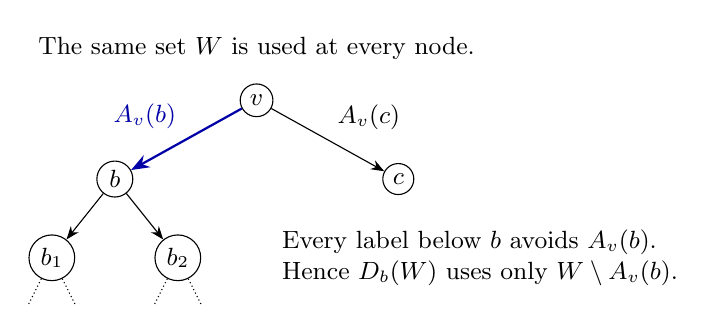
\begin{tikzpicture}[x=1cm,y=1cm,>=Stealth,
  vertex/.style={circle,draw,fill=white,inner sep=2pt},
  every node/.style={font=\small}]
\node[vertex] (v) at (0,0) {$v$};
\node[vertex] (b) at (-1.8,-1.0) {$b$};
\node[vertex] (c) at (1.8,-1.0) {$c$};
\node[vertex] (b1) at (-2.6,-2.0) {$b_1$};
\node[vertex] (b2) at (-1.0,-2.0) {$b_2$};
\draw[->,thick,blue!65!black] (v)--node[above left] {$A_v(b)$} (b);
\draw[->] (v)--node[above right] {$A_v(c)$} (c);
\draw[->] (b)--(b1);
\draw[->] (b)--(b2);
\draw[densely dotted] (b1)--(-2.9,-2.6);
\draw[densely dotted] (b1)--(-2.3,-2.6);
\draw[densely dotted] (b2)--(-1.3,-2.6);
\draw[densely dotted] (b2)--(-0.7,-2.6);
\node[align=left,anchor=west] at (0.2,-2.0)
  {Every label below $b$ avoids $A_v(b)$.\\
   Hence $D_b(W)$ uses only $W\setminus A_v(b)$.};
\node[anchor=south] at (0,0.4) {The same set $W$ is used at every node.};
\end{tikzpicture}
\caption{Every arc below $b$ lies on a path through the arc into $b$, so
$D_b$ is a function of coordinates outside the incoming label. The
diagram is schematic; labels on different branches may overlap.}
\label{fig:outside}
\end{figure}

\step{Step 4 (expected potential, one level).} Now let $W\sim\mu_\rho$.
Let $v$ have outgoing level $j$. Taking expectations in
\eqref{eq:pruning-recurrence},
\[
 \epsilon_j\,\EE D_v(W)=\EE d_v(W)+\sum_{b\in\ch(v)}\EE\bigl[t_{vb}(W)D_b(W)\bigr].
\]
\emph{First term.} $\EE d_v(W)$ is the probability of local failure at
$v$, so $\EE d_v(W)\le\ee^{-9m_j}$ by \eqref{eq:local-failure}.

\emph{Second term.} Non-failure requires $Z_v(Y)\ge\ee^{-10m_j}$, hence
\[
 t_{vb}(W)\le
 \PP\bigl(\mathrm{target}=b,\ Z_v(Y)\ge\ee^{-10m_j}\mid W\bigr).
\]
Multiply by $D_b(W)\ge0$ and take expectations. Then apply
\eqref{eq:distortion} with $f=D_b$. By Step~3, $D_b(W)$ depends only on
$W\setminus A_v(b)$, which is exactly the case in which Step~6 of the
proof of Lemma~\ref{lem:local} is complete. This gives
\[
 \EE\bigl[t_{vb}(W)D_b(W)\bigr]\le\ee^{11m_j}\,\nu_v(b)\,\EE D_b(W).
\]
Dividing by $\epsilon_j=\ee^{-m_j}$,
\begin{equation}\label{eq:expected-potential}
 \EE D_v(W)
 \le \ee^{-8m_j}
    +\ee^{12m_j}\sum_{b\in\ch(v)}\nu_v(b)\,\EE D_b(W).
\end{equation}
This is the step that controls the dependence caused by reusing $W$.

\step{Step 5 (the root is bad with probability below $1/4$).} For
$1\le j\le k+1$ put
\[
 \beta_j=\sum_{i=j}^k
 \exp\Bigl(12\sum_{g=j}^{i-1}m_g-8m_i\Bigr),
 \qquad\text{so that}\qquad
 \beta_{k+1}=0,\quad \beta_j=\ee^{-8m_j}+\ee^{12m_j}\beta_{j+1}.
\]
\emph{Claim: $\EE D_v(W)\le\beta_j$ for every node $v$ with outgoing
level $j$,} where leaves are assigned $j=k+1$. For leaves this is
$0\le0$. If it holds for the children of $v$, then
\eqref{eq:expected-potential} and $\sum_b\nu_v(b)=1$ give
$\EE D_v\le\ee^{-8m_j}+\ee^{12m_j}\beta_{j+1}=\beta_j$.

For the root $o$, Step~2 and Markov's inequality give
\[
 \PP(o\text{ is bad})\le\PP(D_o(W)>1)\le\EE D_o(W)\le\beta_1
 =\sum_{i=1}^k\exp\Bigl(12\sum_{g<i}m_g-8m_i\Bigr).
\]
Since $m_g\le16^{-(i-g)}m_i$, we have
$\sum_{g<i}m_g\le m_i\sum_{x\ge1}16^{-x}=m_i/15$, so the $i$-th exponent
is at most $(12/15-8)m_i\le-7m_i$. The $m_i$ are strictly increasing
positive integers, hence distinct, and
\[
 \beta_1\le\sum_{x\ge1}\ee^{-7x}=\frac1{\ee^{7}-1}<\frac14 .
\]
So the procedure succeeds with probability greater than $3/4$.

\step{Step 6 (the reduced tree; capacity, disjointness, recovery).} Fix
$W$ for which the root is good. Starting from the root, at each retained
good node $v$ with outgoing level $j$ put
\[
 \gamma_v(W)=\sum_{b\ \mathrm{good}}t_{vb}(W)\ge1-\epsilon_j>0 .
\]
Retain each good child $b$ with $t_{vb}(W)>0$, give it weight
$t_{vb}(W)/\gamma_v(W)$, replace its incoming label by
\[
 T_b=A_v(b)\setminus W,
\]
and continue recursively into $b$. Call the result $\TT'$.
\begin{itemize}[leftmargin=2em,itemsep=2pt]
 \item \emph{$\TT'$ is a probability tree with $k$ levels.} The new
 weights at $v$ are positive and sum to one. Since $\gamma_v>0$, every
 retained non-leaf node has a retained child, and retained children are
 good, so the recursion reaches depth $k$.
 \item \emph{Disjoint.} $\TT'$ is a subtree of $\TT$ and each new label
 is a subset of the old one.
 \item \emph{Recovery (ii).} A path $Q$ of $\TT'$ passes through the
 same nodes as a path $P$ of $\TT$. On each arc,
 $A_v(b)\subseteq W\cup T_b$, so $\UU(P)\subseteq W\cup\UU(Q)$.
 \item \emph{Capacity.} If $b$ is retained then $t_{vb}(W)>0$, so some
 non-failing outcome has target $b$. Its fragment is
 $A_v(b)\setminus W=T_b$ and satisfies $|T_b|\le m_j/2$. As $|T_b|$ is
 an integer, $|T_b|\le\lfloor m_j/2\rfloor$.
\end{itemize}

\step{Step 7 (spread of the reduced tree).} Let $v$ be a retained node
with outgoing level $j$, and consider the transition at $v$ for the
fixed $W$. Let $E_v$ be the event ``no local failure and the target is
good''; then $\PP(E_v\mid W)=\gamma_v(W)$. The new child law
$b\mapsto t_{vb}(W)/\gamma_v(W)$ is the law of the target conditioned on
$E_v$, and the new label of the target is the fragment $T$. By
\eqref{eq:two-inclusions}, $T\subseteq A_v(c)$, where $c$ is the source.
The source has law $\nu_v$ at fixed $W$. Hence, for every nonempty
$J\subseteq X$,
\begin{align*}
 \PP(J\subseteq T\mid E_v,W)
 =\frac{\PP(J\subseteq T,\ E_v\mid W)}{\gamma_v(W)}
 &\le\frac{\PP_{c\sim\nu_v}(J\subseteq A_v(c))}{\gamma_v(W)}\\
 &\le\frac{\alpha_j^{|J|}}{1-\epsilon_j}
 \le\left(\frac{\alpha_j}{1-\epsilon_j}\right)^{|J|},
\end{align*}
using $|J|\ge1$ and $0<1-\epsilon_j\le1$ in the last step. This is (i).

\medskip
The numbers $t_{vb}(W)$ determine the whole construction, so the
procedure is deterministic given $W$. Sources and targets are auxiliary
random variables used only to analyse the weights.
\end{proof}

\subsection{Iteration: proof of Theorem~\ref{thm:tree}}

\begin{proof}[Proof of Theorem~\ref{thm:tree}]
\emph{Plan.} Apply Lemma~\ref{lem:reduction} repeatedly with fresh
independent sets of law $\mu_\rho$. Each success halves all capacities,
so after about $\log_2\ell_k$ successes all labels are empty and the
union of the sets used covers a path. Count the attempts and bound the
density of the union.

\step{Step 0 (parameters).} If $r=1$ then $W=X$ almost surely and the
conclusion holds, since $\TT$ has at least one path. Suppose $r<1$, and
set
\[
 a=4\sigma,\qquad \rho=\ee^{50}a,
 \qquad s=\lfloor\log_2\ell_k\rfloor+1.
\]
Then $0<\rho=4\ee^{50}\sigma\le\frac14\cdot16\ee^{50}\sigma(1+\log_2\ell_k)
=r/4<1$.

\step{Step 1 (the process and its invariants).} Start with $\TT_0=\TT$.
Make successive \emph{attempts}: draw a fresh independent set of law
$\mu_\rho$ and run the procedure of Lemma~\ref{lem:reduction} on the
current tree. A failed attempt leaves the current tree unchanged. After
the $\tau$-th success the current tree is replaced by a tree $\TT_\tau$
defined in Step~3; let $W_1,W_2,\ldots$ be the draws of the successful
attempts. Conditionally on the complete past, the current tree is fixed
and the next draw has law $\mu_\rho$. Define, for each original level
$i$,
\begin{equation}\label{eq:capacities}
 m_i(\tau)=\left\lfloor\frac{\ell_i}{2^\tau}\right\rfloor,
 \qquad
 \alpha_i(\tau)=\sigma
 \prod_{u=0}^{\tau-1}
 \left(1-\ee^{-\lfloor\ell_i/2^u\rfloor}\right)^{-1}.
\end{equation}
We maintain the following invariants after $\tau$ successes.
\begin{enumerate}[label=(I\arabic*),leftmargin=2.6em,itemsep=2pt]
 \item $\TT_\tau$ is a disjoint probability tree whose levels are the
 original levels $i$ with $m_i(\tau)\ge1$. Level $i$ has capacity
 $m_i(\tau)$ and is $\alpha_i(\tau)$-spread.
 \item For every path $Q$ of $\TT_\tau$ there is a path $P$ of $\TT$
 with $\UU(P)\subseteq W_1\cup\cdots\cup W_\tau\cup\UU(Q)$.
\end{enumerate}
Since $\ell_i$ increases with $i$, the levels with $m_i(\tau)=0$ form an
initial segment. If no level remains, $\TT_\tau$ is a single node and
the process is \emph{complete}. For $\tau=0$ both invariants hold by
hypothesis.

\step{Step 2 (the hypotheses of Lemma~\ref{lem:reduction} hold for
$\TT_\tau$).} Assume (I1) and that at least one level remains.
\begin{itemize}[leftmargin=2em,itemsep=2pt]
 \item \emph{Capacities.} The remaining $m_i(\tau)$ are positive
 integers, and
 $m_{i+1}(\tau)=\lfloor\ell_{i+1}/2^\tau\rfloor
 \ge\lfloor16\ell_i/2^\tau\rfloor\ge16\lfloor\ell_i/2^\tau\rfloor
 =16m_i(\tau)$, using $\lfloor16x\rfloor\ge16\lfloor x\rfloor$.
 \item \emph{Spread: $\alpha_i(\tau)\le a$.} For a remaining level $i$
 the integers $x_u=\lfloor\ell_i/2^u\rfloor$, $0\le u\le\tau-1$, satisfy
 $x_u\ge m_i(\tau)\ge1$ and
 $x_{u+1}=\lfloor x_u/2\rfloor<x_u$, so they are distinct positive
 integers. Every factor $(1-\ee^{-x})^{-1}$ is at least $1$, so the
 product in \eqref{eq:capacities} is at most
 $\prod_{x\ge1}(1-\ee^{-x})^{-1}$. Using
 $-\log(1-y)=\log\bigl(1+\tfrac y{1-y}\bigr)\le\tfrac y{1-y}$ with
 $y=\ee^{-x}\le\ee^{-1}$,
 \begin{equation}\label{eq:spread-iteration}
 \sum_{x=1}^{\infty}-\log(1-\ee^{-x})
 \le \frac{1}{1-\ee^{-1}}\sum_{x=1}^{\infty}\ee^{-x}
 =\frac{\ee^{-1}}{(1-\ee^{-1})^2}<0.93<\log 4 .
 \end{equation}
 Hence $\alpha_i(\tau)<4\sigma=a$.
 \item $\rho=\ee^{50}a<1$ by Step~0.
\end{itemize}
Therefore every attempt before completion has conditional success
probability at least $3/4$.

\step{Step 3 (one success preserves the invariants).} Suppose the next
attempt on $\TT_\tau$ succeeds with draw $W_{\tau+1}$, and let $\TT'$ be
the tree returned by Lemma~\ref{lem:reduction}. By part~(i), level $i$
of $\TT'$ has capacity
$\lfloor m_i(\tau)/2\rfloor=m_i(\tau+1)$, using
$\lfloor\lfloor x\rfloor/2\rfloor=\lfloor x/2\rfloor$, and is
$\alpha_i(\tau)/(1-\ee^{-m_i(\tau)})=\alpha_i(\tau+1)$-spread.

\emph{Trimming.} The levels of $\TT'$ with $m_i(\tau+1)=0$ form an
initial segment, and all their labels are empty. By a fixed tie-breaking
rule choose a node $o'$ of $\TT'$ at the bottom of this segment, and let
$\TT_{\tau+1}$ be the subtree of $\TT'$ rooted at $o'$. Child laws and
labels at retained nodes are unchanged, so (I1) holds for $\tau+1$. If
no level remains, $\TT_{\tau+1}$ is the single node $o'$.

\emph{Recovery.} Let $Q$ be a path of $\TT_{\tau+1}$. Prepending the
path from the root of $\TT'$ to $o'$ gives a path $Q'$ of $\TT'$ with
$\UU(Q')=\UU(Q)$, because the prefix labels are empty. By
\eqref{eq:recovery} there is a path $Q''$ of $\TT_\tau$ with
$\UU(Q'')\subseteq W_{\tau+1}\cup\UU(Q)$. By (I2) for $\tau$ there is a
path $P$ of $\TT$ with
$\UU(P)\subseteq W_1\cup\cdots\cup W_\tau\cup\UU(Q'')$. Combining gives
(I2) for $\tau+1$.

\step{Step 4 (completion within $s$ successes).} Since
$2^s>2^{\log_2\ell_k}=\ell_k\ge\ell_i$, we have $m_i(s)=0$ for every
$i$. So the process is complete after at most $s$ successes. At
completion the unique path $Q$ of the current tree has
$\UU(Q)=\varnothing$, and (I2) gives a path $P$ of $\TT$ with $\UU(P)$
contained in the union of the successful draws.

\step{Step 5 (number of attempts).} Let $\eta$ be the total number of
attempts until completion. For $1\le u\le s$ let $G_u$ be the number of
attempts after the $(u-1)$-th success up to and including the $u$-th,
with $G_u=0$ if the process is already complete. By Step~2,
conditionally on the past each attempt succeeds with probability at
least $3/4$, so $\PP(G_u>x)\le4^{-x}$ and
$\EE G_u=\sum_{x\ge0}\PP(G_u>x)\le4/3$. Hence
$\EE\eta\le\sum_{u\le s}\EE G_u\le4s/3$, and by Markov's inequality
\[
 \PP(\eta>4s)\le\PP(\eta\ge4s)\le\frac{4s/3}{4s}=\frac13 .
\]

\step{Step 6 (the union of the draws).} Predraw $4s$ independent sets
of law $\mu_\rho$, use them in order as the attempts, and let $W_*$ be
the union of all $4s$ sets, including any not used. Each element of $X$
lies in $W_*$ independently with probability
\[
 r_*=1-(1-\rho)^{4s}
 \le4s\rho
 =16\ee^{50}\sigma s
 \le16\ee^{50}\sigma(1+\log_2\ell_k)=r,
\]
by Bernoulli's inequality, and using
$s\le1+\log_2\ell_k$ and $r<1$. So $W_*\sim\mu_{r_*}$. On the event
$\eta\le4s$, which has probability at least $2/3$, Step~4 shows that
$W_*$ contains $\UU(P)$ for some path $P$ of $\TT$. The event
``$W\supseteq\UU(P)$ for some $P$'' is increasing in $W$, and for
$r_*\le r$ a set of law $\mu_{r_*}$ can be coupled inside a set of law
$\mu_r$: take $W_p=\{x:U_x\le p\}$ for independent uniform variables
$U_x$. Hence the same bound holds for $\mu_r$.
\end{proof}

\section{Application to graph containment}\label{sec:graphs}

It remains to construct, from $H$, a tree satisfying the hypotheses of
Theorem~\ref{thm:tree}. The construction is the normalized-containment
maximization and conditional-extension argument of
Tran~\cite[Section~3, Lemma~3.1]{Tran26}, with constants suited to the
factor-$16$ separation of capacities. The identity
\eqref{eq:copy-ratio} below also appears
in~\cite[Equation~(5)]{MNSZ22}.

\subsection{Conventions for copies}

Put
\[
 q=\pE(n,H),\qquad \sigma=128q,\qquad X=\tbinom{[n]}2 .
\]
By fact~(b) of Section~\ref{sec:introduction}, $q>0$. The number $q$ is
always defined from the original graph $H$.

\emph{Isolated vertices.} Delete the isolated vertices of $H$ and of
every graph considered below, and identify each such graph with its edge
set; in particular $H$ now also denotes its edge set and $|H|=e(H)=h$.
If a graph on $[n]$ contains a copy of $H$ without its isolated
vertices, it contains a copy of $H$: add the required number of unused
vertices, which exist since $n\ge|V(H)|$ and copies need not be induced.

\emph{Copies.} For an edge set $F$ on at most $n$ vertices, a
\emph{copy of $F$ on $[n]$} is a set $F_0\subseteq X$ whose edges form a
graph isomorphic to $F$. Let
\[
 M(F)=N(K_n,F)=\#\{\text{copies of }F\text{ on }[n]\},\qquad
 M(I,F)=N(I,F)=\#\{F'\subseteq I:\ F'\cong F\},
\]
with $M(\varnothing)=M(I,\varnothing)=1$. Explicitly,
$M(F)=(n)_{v(F)}/|\operatorname{Aut}(F)|$ with
$(n)_v=n(n-1)\cdots(n-v+1)$; the formula is not needed. Any two copies
of $F$ on $[n]$ differ by a permutation of $[n]$.

\emph{The expectation constraint.} If $S\subseteq H$ is a nonempty edge
subset, then $S$ on its incident vertices is a subgraph of the original
$H$. Since the infimum defining $q$ is attained (fact~(a)),
\eqref{eq:first-moment} gives
\begin{equation}\label{eq:constraint}
 M(S)\,q^{|S|}\ge\tfrac12 .
\end{equation}

\emph{The copy-count identity.} Let $\boldsymbol I$ be a uniformly
chosen copy of $I$ on $[n]$, and let $F_0$ be a fixed copy of an edge
subset $F\subseteq I$. Then
\begin{equation}\label{eq:copy-ratio}
 \PP(F_0\subseteq\boldsymbol I)=\frac{M(I,F)}{M(F)}.
\end{equation}
Indeed, the law of $\boldsymbol I$ is invariant under permutations of
$[n]$, so the probability is the same for every copy $F_0$. Summing over
all $M(F)$ copies gives the expected number of copies of $F$ inside
$\boldsymbol I$, which is $M(I,F)$.

\subsection{The hierarchy}

\begin{lemma}[Graph hierarchy]\label{lem:hierarchy}
There is a disjoint probability tree on $X=\binom{[n]}2$ whose path
unions are copies of $H$ with its isolated vertices removed, such that
every level is $\sigma$-spread and its label sizes
$\ell_1,\ldots,\ell_k$ satisfy
\[
 1\le\ell_1,\qquad \ell_{i+1}\ge16\ell_i,
 \qquad \ell_k\le e(H).
\]
\end{lemma}

\emph{Where it is used.} In the proof of Theorem~\ref{thm:main}, as the
input to Theorem~\ref{thm:tree}.

\begin{proof}
\emph{Plan.} For an edge set $I$, pick the subset $S$ that is ``most
over-represented'' in a random copy of $I$ after discounting by
$\sigma^{|S|}$. Step~1 shows $S$ is much smaller than $I$. Iterating
gives a chain (Step~2) and a tree of copies (Step~3). Maximality of $S$
is exactly the spread condition for extensions (Step~4).

\step{Step 1 (the maximizer is small).} For a nonempty edge set
$I\subseteq H$ and an edge subset $S\subseteq I$, define
\begin{equation}\label{eq:maximizer}
 R_\sigma(I,S)=\sigma^{-|S|}\,\PP(S_0\subseteq\boldsymbol I),
\end{equation}
where $\boldsymbol I$ is a uniform copy of $I$ on $[n]$ and $S_0$ is any
fixed copy of $S$. By \eqref{eq:copy-ratio} this does not depend on the
choice of $S_0$. Choose $S$ maximizing $R_\sigma(I,S)$, with a fixed
deterministic tie-breaking rule. The empty set is allowed and has
$R_\sigma(I,\varnothing)=1$.

\emph{Claim: every maximizer satisfies $|S|<|I|/17$.} Let
$S\subseteq I$ be nonempty. By \eqref{eq:copy-ratio}, the bound
$M(I,S)\le\binom{|I|}{|S|}$ (copies of $S$ in $I$ are $|S|$-subsets of
$I$), and \eqref{eq:constraint} in the form $1/M(S)\le2q^{|S|}$,
\[
 R_\sigma(I,S)=\sigma^{-|S|}\frac{M(I,S)}{M(S)}
 \le2\binom{|I|}{|S|}\Bigl(\frac q\sigma\Bigr)^{|S|}
 =2\binom{|I|}{|S|}128^{-|S|}.
\]
If $|S|\ge|I|/17$, the standard bound
$\binom Nx\le(\ee N/x)^x$ gives
$\binom{|I|}{|S|}\le(17\ee)^{|S|}$, and so, as $|S|\ge1$ and
$17\ee/128<0.362$,
\[
 R_\sigma(I,S)\le2\,(17\ee/128)^{|S|}\le2\cdot0.362<1
 =R_\sigma(I,\varnothing).
\]
Such an $S$ is not a maximizer. In particular the maximizer is a proper
subset of $I$.

\step{Step 2 (the chain).} Start from $I=H$ and apply Step~1
repeatedly, each time replacing $I$ by its maximizer, until the empty
set is reached; this happens because sizes strictly decrease. Writing
the sequence in reverse order,
\[
 \varnothing=H_0\subset H_1\subset\cdots\subset H_k=H,
 \qquad |H_{i-1}|<|H_i|/17,\qquad k\ge1,
\]
where $H_{i-1}$ maximizes $R_\sigma(H_i,\cdot)$.

\step{Step 3 (the tree).} The root is the empty edge set. A node at
depth $i$ is a history $(S^{(0)},\ldots,S^{(i)})$ with
$\varnothing=S^{(0)}\subset S^{(1)}\subset\cdots\subset S^{(i)}$ and
$S^{(g)}$ a copy of $H_g$ on $[n]$. Distinct histories are distinct
nodes. The children of a node ending in the copy $S_0$ of $H_{i-1}$ are
obtained by appending any copy $I_0$ of $H_i$ with $I_0\supseteq S_0$.
The child law is uniform, and the arc label is $I_0\setminus S_0$.
\begin{itemize}[leftmargin=2em,itemsep=2pt]
 \item \emph{Children exist.} Take any copy $I_1$ of $H_i$ on $[n]$. It
 contains a copy of $H_{i-1}$, which some permutation $\phi$ of $[n]$
 maps to $S_0$. Then $\phi(I_1)$ is a copy of $H_i$ containing $S_0$.
 So all leaves have depth $k$.
 \item \emph{Disjointness and path unions.} Along a path the labels are
 $S^{(g)}\setminus S^{(g-1)}$, $1\le g\le k$. They are pairwise disjoint
 and their union is $S^{(k)}$, a copy of $H_k=H$.
 \item \emph{Sizes.} Every label on level $i$ has size
 $\ell_i=|H_i|-|H_{i-1}|>0$. Thus $\ell_1\ge1$,
 $\ell_k\le|H_k|=e(H)$, and
 \[
  \ell_{i+1}=|H_{i+1}|-|H_i|>17|H_i|-|H_i|=16|H_i|\ge16\ell_i .
 \]
\end{itemize}

\step{Step 4 (every level is $\sigma$-spread).} Fix a node at depth
$i-1$ ending in the copy $S_0$ of $H_{i-1}$. Let $\boldsymbol I$ be a
uniform copy of $H_i$ on $[n]$. The child law is the law of
$\boldsymbol I$ conditioned on $\{S_0\subseteq\boldsymbol I\}$, and the
label is $A=\boldsymbol I\setminus S_0$. Let $J\subseteq X$ be nonempty.

If $J\cap S_0\ne\varnothing$, then $\PP(J\subseteq A)=0$. Otherwise
\begin{equation}\label{eq:conditional-ratio}
 \PP(J\subseteq A)=
 \frac{\PP(S_0\cup J\subseteq\boldsymbol I)}
      {\PP(S_0\subseteq\boldsymbol I)}.
\end{equation}
If the numerator is zero the bound $\PP(J\subseteq A)\le\sigma^{|J|}$ is
trivial. If it is positive, $S_0\cup J$ lies in a copy of $H_i$, so it
is a copy of some edge subset $S'\subseteq H_i$ with
$|S'|=|S_0|+|J|$. Maximality of $H_{i-1}$, that is
$R_\sigma(H_i,S')\le R_\sigma(H_i,H_{i-1})$, reads
\[
 \sigma^{-(|S_0|+|J|)}\PP(S_0\cup J\subseteq\boldsymbol I)
 \le \sigma^{-|S_0|}\PP(S_0\subseteq\boldsymbol I).
\]
Dividing and using \eqref{eq:conditional-ratio} gives
$\PP(J\subseteq A)\le\sigma^{|J|}$. This is \eqref{eq:spread} with
$a=\sigma$.
\end{proof}

\subsection{Proof of the main theorem}

\begin{proof}[Proof of Theorem~\ref{thm:main}]
\emph{Step 1.} The tree of Lemma~\ref{lem:hierarchy} satisfies the
hypotheses of Theorem~\ref{thm:tree} with $\sigma=128q>0$ and capacities
$\ell_1,\ldots,\ell_k$. With
$r=\min\{1,16\ee^{50}\cdot128q(1+\log_2\ell_k)\}$, a set $W\sim\mu_r$
contains the label union of some path with probability at least $2/3$.
Such a union is a copy of $H$ without isolated vertices, and $W$ is the
edge set of $G(n,r)$. By the convention on isolated vertices in
Section~\ref{sec:graphs},
$\PP(N(G(n,r),H)>0)\ge2/3$.

\emph{Step 2.} Since $\ell_k\le h$,
\[
 r\le r':=\min\{1,\;2048\ee^{50}q(1+\log_2 h)\}.
\]
Containing $H$ is an increasing event, so
$\PP(N(G(n,r'),H)>0)\ge2/3\ge1/2$, by the same coupling as in Step~6 of
the proof of Theorem~\ref{thm:tree}. Hence $\pc(n,H)\le r'$, which is
\eqref{eq:stronger}.

\emph{Step 3.} Finally $h\le\binom n2\le n^2$ and $\log_2n\ge1$ give
$1+\log_2h\le1+2\log_2n\le3\log_2n$, hence
$\pc(n,H)\le3\cdot2048\,\ee^{50}q\log_2n=6144\ee^{50}\pE(n,H)\log_2n$.
\end{proof}

\section{Verification checklist}

The following steps carry the argument. A sceptical reader should check
them first.

\begin{enumerate}[label=\arabic*.,leftmargin=2em,itemsep=3pt]
 \item \textbf{The flagged statement.} Inequality \eqref{eq:distortion}
 is false for arbitrary $f(W)$ (remark after Lemma~\ref{lem:local}). It
 is proved for $f$ depending only on $W\setminus A_b$
 (Lemma~\ref{lem:local}, Step~6). Check that its single application,
 Lemma~\ref{lem:reduction} Step~4 with $f=D_b$, is of that form; this is
 Lemma~\ref{lem:reduction}, Step~3.
 \item \textbf{Disjointness makes $D_b$ independent of the incoming
 label.} Lemma~\ref{lem:reduction}, Step~3, using locality (T3) and the
 fact that every arc below $b$ lies on a path through $(v,b)$. This is
 the only place where disjointness along paths is essential.
 \item \textbf{Density identity and local failure bound.} (T4),
 equation \eqref{eq:density}, and Lemma~\ref{lem:local}, Steps~1--5; the
 arithmetic is $\ee^{10m}2^m\ee^{-25m}\le\ee^{-10m}$ and
 $2\ee^{-10m}\le\ee^{-9m}$.
 \item \textbf{The potential argument.} Bad nodes have $D_v>1$
 (Lemma~\ref{lem:reduction}, Step~2). The recursion
 \eqref{eq:expected-potential} and its solution, with
 $12/15-8\le-7$ coming from $m_{j+1}\ge16m_j$
 (Lemma~\ref{lem:reduction}, Steps~4--5).
 \item \textbf{Spread survives the reduction.} The fragment lies inside
 the source label, and the source keeps law $\nu_v$ at fixed $W$
 (Lemma~\ref{lem:reduction}, Step~7).
 \item \textbf{Iteration bookkeeping.} The accumulated spread loss is
 below $4$, by \eqref{eq:spread-iteration}, so the hypothesis
 $\alpha\le a=4\sigma$ of Lemma~\ref{lem:reduction} holds at every stage
 (Theorem~\ref{thm:tree}, Step~2). Trimming empty levels preserves
 recovery (Step~3). $\PP(\eta>4s)\le1/3$ and $r_*\le4s\rho\le r$
 (Steps~5--6).
 \item \textbf{The graph input.} Maximizers are small, using
 \eqref{eq:constraint}, i.e.\ the definition of $\pE$, and
 $2\cdot17\ee/128<1$ (Lemma~\ref{lem:hierarchy}, Step~1). Maximality
 gives $\sigma$-spread (Lemma~\ref{lem:hierarchy}, Step~4).
 \item \textbf{Constants.} $16\cdot128=2048$ and
 $1+\log_2h\le3\log_2n$ (proof of Theorem~\ref{thm:main}, Steps~2--3).
\end{enumerate}

\begin{thebibliography}{99}
\raggedright

\bibitem{ALWZ21}
R.~Alweiss, S.~Lovett, K.~Wu, and J.~Zhang,
\emph{Improved bounds for the sunflower lemma},
Annals of Mathematics (2) \textbf{194} (2021), no.~3, 795--815.
\href{https://doi.org/10.4007/annals.2021.194.3.5}{doi:10.4007/annals.2021.194.3.5}.

\bibitem{Bollobas81}
B.~Bollob\'as,
\emph{Threshold functions for small subgraphs},
Mathematical Proceedings of the Cambridge Philosophical Society
\textbf{90} (1981), no.~2, 197--206.
\href{https://doi.org/10.1017/S0305004100058655}{doi:10.1017/S0305004100058655}.

\bibitem{DKP25}
Q.~Dubroff, J.~Kahn, and J.~Park,
\emph{On the ``second'' Kahn--Kalai conjecture},
arXiv:2508.14269v1 (August 19, 2025).
\url{https://arxiv.org/abs/2508.14269v1}.

\bibitem{DKP25Cases}
Q.~Dubroff, J.~Kahn, and J.~Park,
\emph{On the ``second'' Kahn--Kalai conjecture: cliques, cycles, and trees},
arXiv:2510.02005v2 (October 23, 2025).
\url{https://arxiv.org/abs/2510.02005v2}.

\bibitem{ER60}
P.~Erd\H{o}s and A.~R\'enyi,
\emph{On the evolution of random graphs},
Publications of the Mathematical Institute of the Hungarian Academy of
Sciences \textbf{5} (1960), 17--61.
\url{https://static.renyi.hu/~p_erdos/1960-10.pdf}.

\bibitem{ER66}
P.~Erd\H{o}s and A.~R\'enyi,
\emph{On the existence of a factor of degree one of a connected random graph},
Acta Mathematica Academiae Scientiarum Hungaricae
\textbf{17} (1966), 359--368.
\url{https://users.renyi.hu/~p_erdos/1966-16.pdf}.

\bibitem{FKNP21}
K.~Frankston, J.~Kahn, B.~Narayanan, and J.~Park,
\emph{Thresholds versus fractional expectation-thresholds},
Annals of Mathematics (2) \textbf{194} (2021), no.~2, 475--495.
\href{https://doi.org/10.4007/annals.2021.194.2.2}{doi:10.4007/annals.2021.194.2.2}.

\bibitem{KK07}
J.~Kahn and G.~Kalai,
\emph{Thresholds and expectation thresholds},
Combinatorics, Probability and Computing
\textbf{16} (2007), no.~3, 495--502.
\href{https://doi.org/10.1017/S0963548307008474}{doi:10.1017/S0963548307008474}.

\bibitem{LSZ19}
S.~Lovett, N.~Solomon, and J.~Zhang,
\emph{From DNF compression to sunflower theorems via regularity},
34th Computational Complexity Conference, LIPIcs \textbf{137} (2019),
5:1--5:14.
\href{https://doi.org/10.4230/LIPIcs.CCC.2019.5}{doi:10.4230/LIPIcs.CCC.2019.5}.

\bibitem{MNSZ25}
E.~Mossel, J.~Niles-Weed, N.~Sun, and I.~Zadik,
\emph{A Bayesian proof of the spread lemma},
Random Structures \& Algorithms \textbf{66} (2025), no.~4, e70008.
\href{https://doi.org/10.1002/rsa.70008}{doi:10.1002/rsa.70008}.

\bibitem{MNSZ22}
E.~Mossel, J.~Niles-Weed, N.~Sun, and I.~Zadik,
\emph{On the second Kahn--Kalai conjecture},
arXiv:2209.03326v1 (September 7, 2022).
\url{https://arxiv.org/abs/2209.03326v1}.

\bibitem{OpenAIThresholdEquivalence2026}
OpenAI,
\emph{Integral and fractional expectation thresholds are equivalent},
OpenAI Math Release preprint
\href{https://github.com/openai/math/blob/main/preprints/Integral-and-fractional-expectation-thresholds-are-equivalent-September-23-2026/paper.pdf}{OAI:Integral-and-fractional-expectation-thresholds-are-equivalent-September-23-2026},
2026, Theorem~1.1, p.~2.

\bibitem{PP24}
J.~Park and H.~T.~Pham,
\emph{A proof of the Kahn--Kalai conjecture},
Journal of the American Mathematical Society
\textbf{37} (2024), no.~1, 235--243.
\href{https://doi.org/10.1090/jams/1028}{doi:10.1090/jams/1028}.

\bibitem{Riordan00}
O.~Riordan,
\emph{Spanning subgraphs of random graphs},
Combinatorics, Probability and Computing
\textbf{9} (2000), no.~2, 125--148.
\href{https://doi.org/10.1017/S0963548399004150}{doi:10.1017/S0963548399004150}.

\bibitem{Tal10}
M.~Talagrand,
\emph{Are many small sets explicitly small?},
Proceedings of the 42nd ACM Symposium on Theory of Computing (2010),
13--36.
\href{https://doi.org/10.1145/1806689.1806693}{doi:10.1145/1806689.1806693}.

\bibitem{Tran26}
T.~Tran,
\emph{Fractional expectation thresholds and the ``second'' Kahn--Kalai
conjecture},
arXiv:2609.20546v2 (September 24, 2026).
\url{https://arxiv.org/abs/2609.20546v2}.

\end{thebibliography}

\end{document}
